% last updated in April 2002 by Antje Endemann
% Based on CVPR 07 and LNCS, with modifications by DAF, AZ and elle, 2008 and AA, 2010, and CC, 2011; TT, 2014; AAS, 2016

\documentclass[runningheads]{llncs}
\usepackage{graphicx}
\usepackage{amsmath,amssymb} % define this before the line numbering.
%\usepackage{ruler}
\usepackage{color}
\usepackage[width=122mm,left=12mm,paperwidth=146mm,height=193mm,top=12mm,paperheight=217mm]{geometry}
\usepackage{cite}

\newcommand{\yty}[1]{\textcolor{black}{#1}}
\newcommand{\ytyy}[1]{\textcolor{black}{#1}}
\newcommand{\abc}[1]{\textcolor{black}{#1}}
\newcommand{\abcn}[1]{\textcolor{black}{#1}}
\newcommand{\abcnote}[1]{\textcolor{magenta}{[NOTE: #1]}}


\begin{document}
% \renewcommand\thelinenumber{\color[rgb]{0.2,0.5,0.8}\normalfont\sffamily\scriptsize\arabic{linenumber}\color[rgb]{0,0,0}}
% \renewcommand\makeLineNumber {\hss\thelinenumber\ \hspace{6mm} \rlap{\hskip\textwidth\ \hspace{6.5mm}\thelinenumber}}
% \linenumbers
%\pagestyle{headings}
%\mainmatter
%\def\ECCV18SubNumber{231}  % Insert your submission number here

\title{Learning Dynamic Memory Networks for Object Tracking} % Replace with your title

%\titlerunning{ECCV-18 submission ID \ECCV18SubNumber}

%\authorrunning{ECCV-18 submission ID \ECCV18SubNumber}

\author{Tianyu Yang\quad Antoni B. Chan}
\institute{Department of Computer Science, City University of Hong Kong\\
\tt\small tianyyang8-c@my.cityu.edu.hk, abchan@cityu.edu.hk}


\maketitle

\begin{abstract}
Template-matching methods for visual tracking have gained popularity recently due to their comparable performance and fast speed. However, they lack effective ways to adapt to changes in the target object's appearance, making their tracking accuracy still far from state-of-the-art. In this paper, we propose a dynamic memory network to adapt the template to the target's appearance variations during tracking. An LSTM is used as a memory controller, where the input is the search feature map and the outputs are the control signals for the reading and writing process of the memory block. As the location of the target is at first unknown in the search feature map, an attention mechanism is applied to concentrate the LSTM input on the potential target. To prevent aggressive model adaptivity, we apply gated residual template learning to control the amount of retrieved memory that is used to combine with the initial template. Unlike tracking-by-detection methods where the object's information is maintained by the weight parameters of neural networks, which requires expensive online fine-tuning to be adaptable, our tracker runs completely feed-forward and adapts to the target's appearance changes by updating the external memory. Moreover, the capacity of our model is not determined by the network size as with other trackers -- the capacity can be easily enlarged as the memory requirements of a task increase, which is favorable for memorizing long-term object information. Extensive experiments on OTB and VOT demonstrates that our tracker MemTrack performs favorably against state-of-the-art tracking methods while retaining real-time speed of 50 fps.

\keywords{Addressable Memory, Gated Residual Template Learning}
\end{abstract}


\section{Introduction}

Along with the success of convolution neural networks in object recognition and detection,  an increasing number of trackers \cite{Song2017, Nam2016, Wang2015, Bertinetto2016, Guo2017} have adopted deep learning models for visual object tracking. Among them are two dominant tracking strategies. One is the {\em tracking-by-detection} scheme that online trains an object appearance classifier \cite{Song2017, Nam2016} to distinguish the target from the background. The model is first learned using the initial frame, and then fine-tuned using the training samples generated in the subsequent frames based on the newly predicted bounding box. The other scheme is {\em template matching}, which adopts either the target patch in the first frame \cite{Bertinetto2016, Tao2016} or the previous frame \cite{Held2016} to construct the matching model. To handle changes in target appearance, % in succeeding frames, 
the template built in the first frame may be interpolated by the recently generated object template with a small learning rate \cite{Valmadre2017}.  

The main difference between these two strategies is that tracking-by-detection maintains the target's appearance information in the weights of the deep neural network, thus requiring online fine-tuning with stochastic gradient descent (SGD) to make the model adaptable,
% needs SGD to account for online adaptivity, 
while in contrast, template matching stores the target's appearance in the object template, which is generated by a feed forward computation.  Due to the computationally expensive model updating required in tracking-by-detection, the speed of such methods are usually slow, e.g.\ %these three algorithms
\cite{Song2017, Nam2016, Nam2016-1} run at about 1 fps,
%\NOTE{can we say "slower than real-time (X fps)"?}, 
although they do achieve state-of-the-art tracking accuracy. 
%\begin{figure}[t]
%	\begin{center}
%		\fbox{\rule{0pt}{2in} \rule{0.9\linewidth}{0pt}}
%		%\includegraphics[width=0.8\linewidth]{egfigure.eps}
%	\end{center}
%	\caption{Insert some figures}
%	\label{fig:1}
%\end{figure}
%
Template matching methods, however, are fast %do not have this drawback 
because there is no need to update the parameters of the neural networks. Recently, several trackers \cite{Bertinetto2016, Guo2017, Yang2017} adopt fully convolutional Siamese networks as the matching model, which demonstrate promising results and real-time speed.  However, there is still a large performance gap between template-matching models and tracking-by-detection, due to the lack of an effective method for adapting to appearance variations online.


In this paper, we propose a dynamic memory network, where the target information is stored and recalled from  external memory,  to maintain the variations of object appearance for template-matching.
% is used for target information reading and writing. 
Unlike tracking-by-detection  where the target's information is stored in the weights of neural networks and therefore the capacity of the model is limited by the number of parameters, the model capacity of our memory networks can be easily enlarged by increasing the size of external memory, which is useful for memorizing long-term appearance variations. 
%
Since aggressive template updating is prone to overfit recent frames and the initial template is the most reliable one,
we use the initial template as a conservative reference of the object and a residual template, %stored in external memory 
obtained from retrieved memory, to adapt to the appearance variations.
%
During tracking, the residual template is %retrieved from external memory and 
\abc{gated channel-wise and} 
combined with the initial template to form the final matching template, which is then convolved with the search image features to get the response map.
\abc{The channel-wise gating of the residual template controls how much each channel of the retrieved template should be added to the initial template, which can be interpreted as a feature/part selector for adapting the template.}
%
An LSTM (Long Short-Term Memory) is used to control the reading and writing process of external memory, 
\abc{as well as the channel-wise gate vector for the residual template.}
 %
% \NOTE{below is a lot of detail for the intro. Cut it down to a few sentences highlighting the important steps and their motivation: attention, channel-wise read keys.}
%Because the object's position on new coming frame is unknown, we adopt an attention mechanism to calculate a soft representation of target by scoring the match degree between the representational vectors around different positions of search feature map and the hidden state of LSTM where historical target's information is stored. This soft feature vector is then feed into LSTM to output the controlling factors for memory access. Moreover, we multiply the reading template by a channel-wise residual vectors output by controller to determine how much new information should be added to the initial template. This helps improve the tracking performance by alleviating model degradation caused by aggressive model adaptivity.
%%It also generates a channel-wise gate vector to control how much of the retrieved template should be added to the initial template for each channel, which can be interpreted as a feature/part selector for adapting the template.
% . This improves the tracking performance, % as is shown in Section \ref{abla}, 
%since it alleviates model degradation caused by aggressive model adaptivity. 
In addition, as the target position is at first unknown in the search image, we adopt an attention mechanism to locate the object roughly % (Figure \ref{fig:3}) 
in the search image, thus leading to a soft representation of the target for the input to the LSTM controller. This helps to retrieve the most-related template in the memory. %for appearance adaptivity. } 
%
%\NOTE{--- end too much detail ---}
The whole framework is differentiable and therefore can be trained end-to-end with SGD. In summary, the contributions of our work are:
\begin{itemize}
	\item We design a dynamic memory network for visual tracking. An external memory block, which is controlled by an LSTM with attention mechanism, allows adaptation to appearance variations. %manages the target's appearance adaptivity.
	\item We propose \abc{gated} residual template learning to generate the final matching template, which effectively controls the amount of appearance variations in retrieved memory that is added to \abc{each channel of} the initial matching template.
	% \NOTE{I could not parse the  last part of this sentence "retried memory adding"}. 
	This prevents excessive model updating, while retaining the conservative information of the target.
	\item We extensively evaluate our algorithm on large scale datasets OTB and VOT. Our tracker performs favorably against state-of-the-art tracking methods while possessing real-time speed of 50 fps.
	%  \NOTE{can you make a stronger statement? outperforms other real-time trackers (template-based?), and performs favorably against non-real time trackers (tracking-by-detection).}
\end{itemize}

\section{Related Work}
\textbf{Template-Matching Trackers}. Matching-based methods have recently gained popularity due to its fast speed and comparable performance. The most notable is the fully convolutional Siamese networks (SiamFC) \cite{Bertinetto2016}. Although it only uses the first frame as the template, SiamFC achieves competitive results and fast speed. The key deficiency of SiamFC is that it lacks an effective model for online updating. 
%, even though its improved version in 
To address this, \cite{Valmadre2017} proposes model updating using linear interpolation of new templates with a small learning rate, but does only sees modest improvements in accuracy.
%
Recently, the RFL (Recurrent Filter Learning) tracker \cite{Yang2017} adopts a convolutional LSTM for model updating, where the forget and input gates control the linear combination of historical target information, \emph{i.e.}, memory states of LSTM, and incoming object's template automatically. Guo \emph{et al.} \cite{Guo2017} propose a dynamic Siamese network with two general transformations for target appearance variation and background suppression.
% transformation. 
To further improve the speed of SiamFC, \cite{Huang2017} 
reduces the feature computation cost for easy frames, by using deep reinforcement learning to train policies for early stopping the feed-forward calculations of the CNN when the response confidence is high enough.
%
%Moreover, 
SINT \cite{Tao2016} also uses Siamese networks for visual tracking and has higher accuracy, but runs much slower than SiamFC (2 fps vs 86 fps) due to the use of deeper CNN (VGG16) for feature extraction, and optical flow for its candidate sampling strategy. Unlike other template-matching models that use sliding windows or random sampling to generate candidate image patches for testing, GOTURN \cite{Held2016} directly regresses the coordinates of the target's bounding box by comparing the previous and current image patches. Despite its advantage on handling scale and aspect ratio changes and fast speed, its tracking accuracy is much lower than other state-of-the-art trackers. 
%\NOTE{using memory is also a major difference. You can also say that you use SiamFC as the baseline feature extractor, since it is the current best template-matching method -- and we extend it to use memory to adapt to variations of apperance.}

Different from existing matching-based trackers where the capacity of adaptivity is limited by the size of neural networks, we use  SiamFC \cite{Bertinetto2016} as the baseline feature extractor and extend it to use an addressable memory, whose memory size is independent of neural networks and thus can be easily enlarged as memory requirements of a task increase, to adapt to variations of object appearance.

\textbf{Memory Networks}. Recent use of convolutional LSTM for visual tracking \cite{Yang2017} shows that memory states %modules 
are useful for object template management over long timescales. Memory networks are typically used to solve simple logical reasoning problem in natural language processing like question answering and sentiment analysis. The pioneering works include NTM (Neural Turing Machine) \cite{Graves2014} and MemNN (Memory Neural Networks) \cite{Weston2015}. They both propose an addressable external memory with reading and writing mechanism -- NTM focuses on problems of sorting, copying and recall, while MemNN aims at language and reasoning task. MemN2N %\NOTE{MemeN2N or MemN2N?} 
\cite{Sukhbaatar2015} further improves MemNN by removing the supervision of supporting facts, which makes it trainable in an end-to-end fashion. Based on their predecessor NTM, %Graves \emph{et al.} 
\cite{Graves2016} proposes a new framework called DNC (Differentiable Neural Computer), which uses a different access mechanism to alleviate the memory overlap and interference problem.
Recently, NTM is also applied to one-shot learning \cite{Santoro2016} by redesigning the method for reading and writing memory, and has shown promising results at %and ability of
encoding and retrieving new information quickly. 

Our proposed memory model differs from the aforementioned memory networks in the following aspects. Firstly, for question answering problem, the input of each time step is a sentence,
% \NOTE{each time step is a sentence input? or each time-step is a word in a sentence? \yty{the first one}}, 
\emph{i.e.}, a sequence of feature vectors (each word corresponds to one vector) which needs an embedding layer (usually RNN) to obtain an internal state. While for object tracking, the input is a search image which needs a feature extraction process (usually CNN) to get a more abstract representation. Furthermore, for object tracking, the target's position in the search image patch is unknown, and here we propose an attention mechanism to highlight the target's information when generating the read key for memory retrieval. 
%
%
Secondly, the dimension of feature vector stored in memory for natural language processing is relatively small (50 in MemN2N vs 6$\times$6$\times$256=9216 in our case). %, even for one-shot learning (image size is only 20x20=400). 
Directly using the original template for address calculation is time-consuming.  Therefore we apply an average pooling on the feature map to generate a template key for addressing, which is efficient and effective experimentally. 
%Furthermore, we apply residual template learning for memory reading and redesign other parts including the way of memory writing and write weight computation to make it more suitable for visual tracking application
Furthermore, we apply \abc{channel-wise gated} residual template learning for model updating, and redesign the memory writing operation %so that %which 
%it is 
to be more suitable for visual tracking.
% \NOTE{this sentence is hard to parse. rewrite it.}.

\section{Dynamic Memory Networks for Tracking}

\begin{figure*}[t]
	\begin{center}
		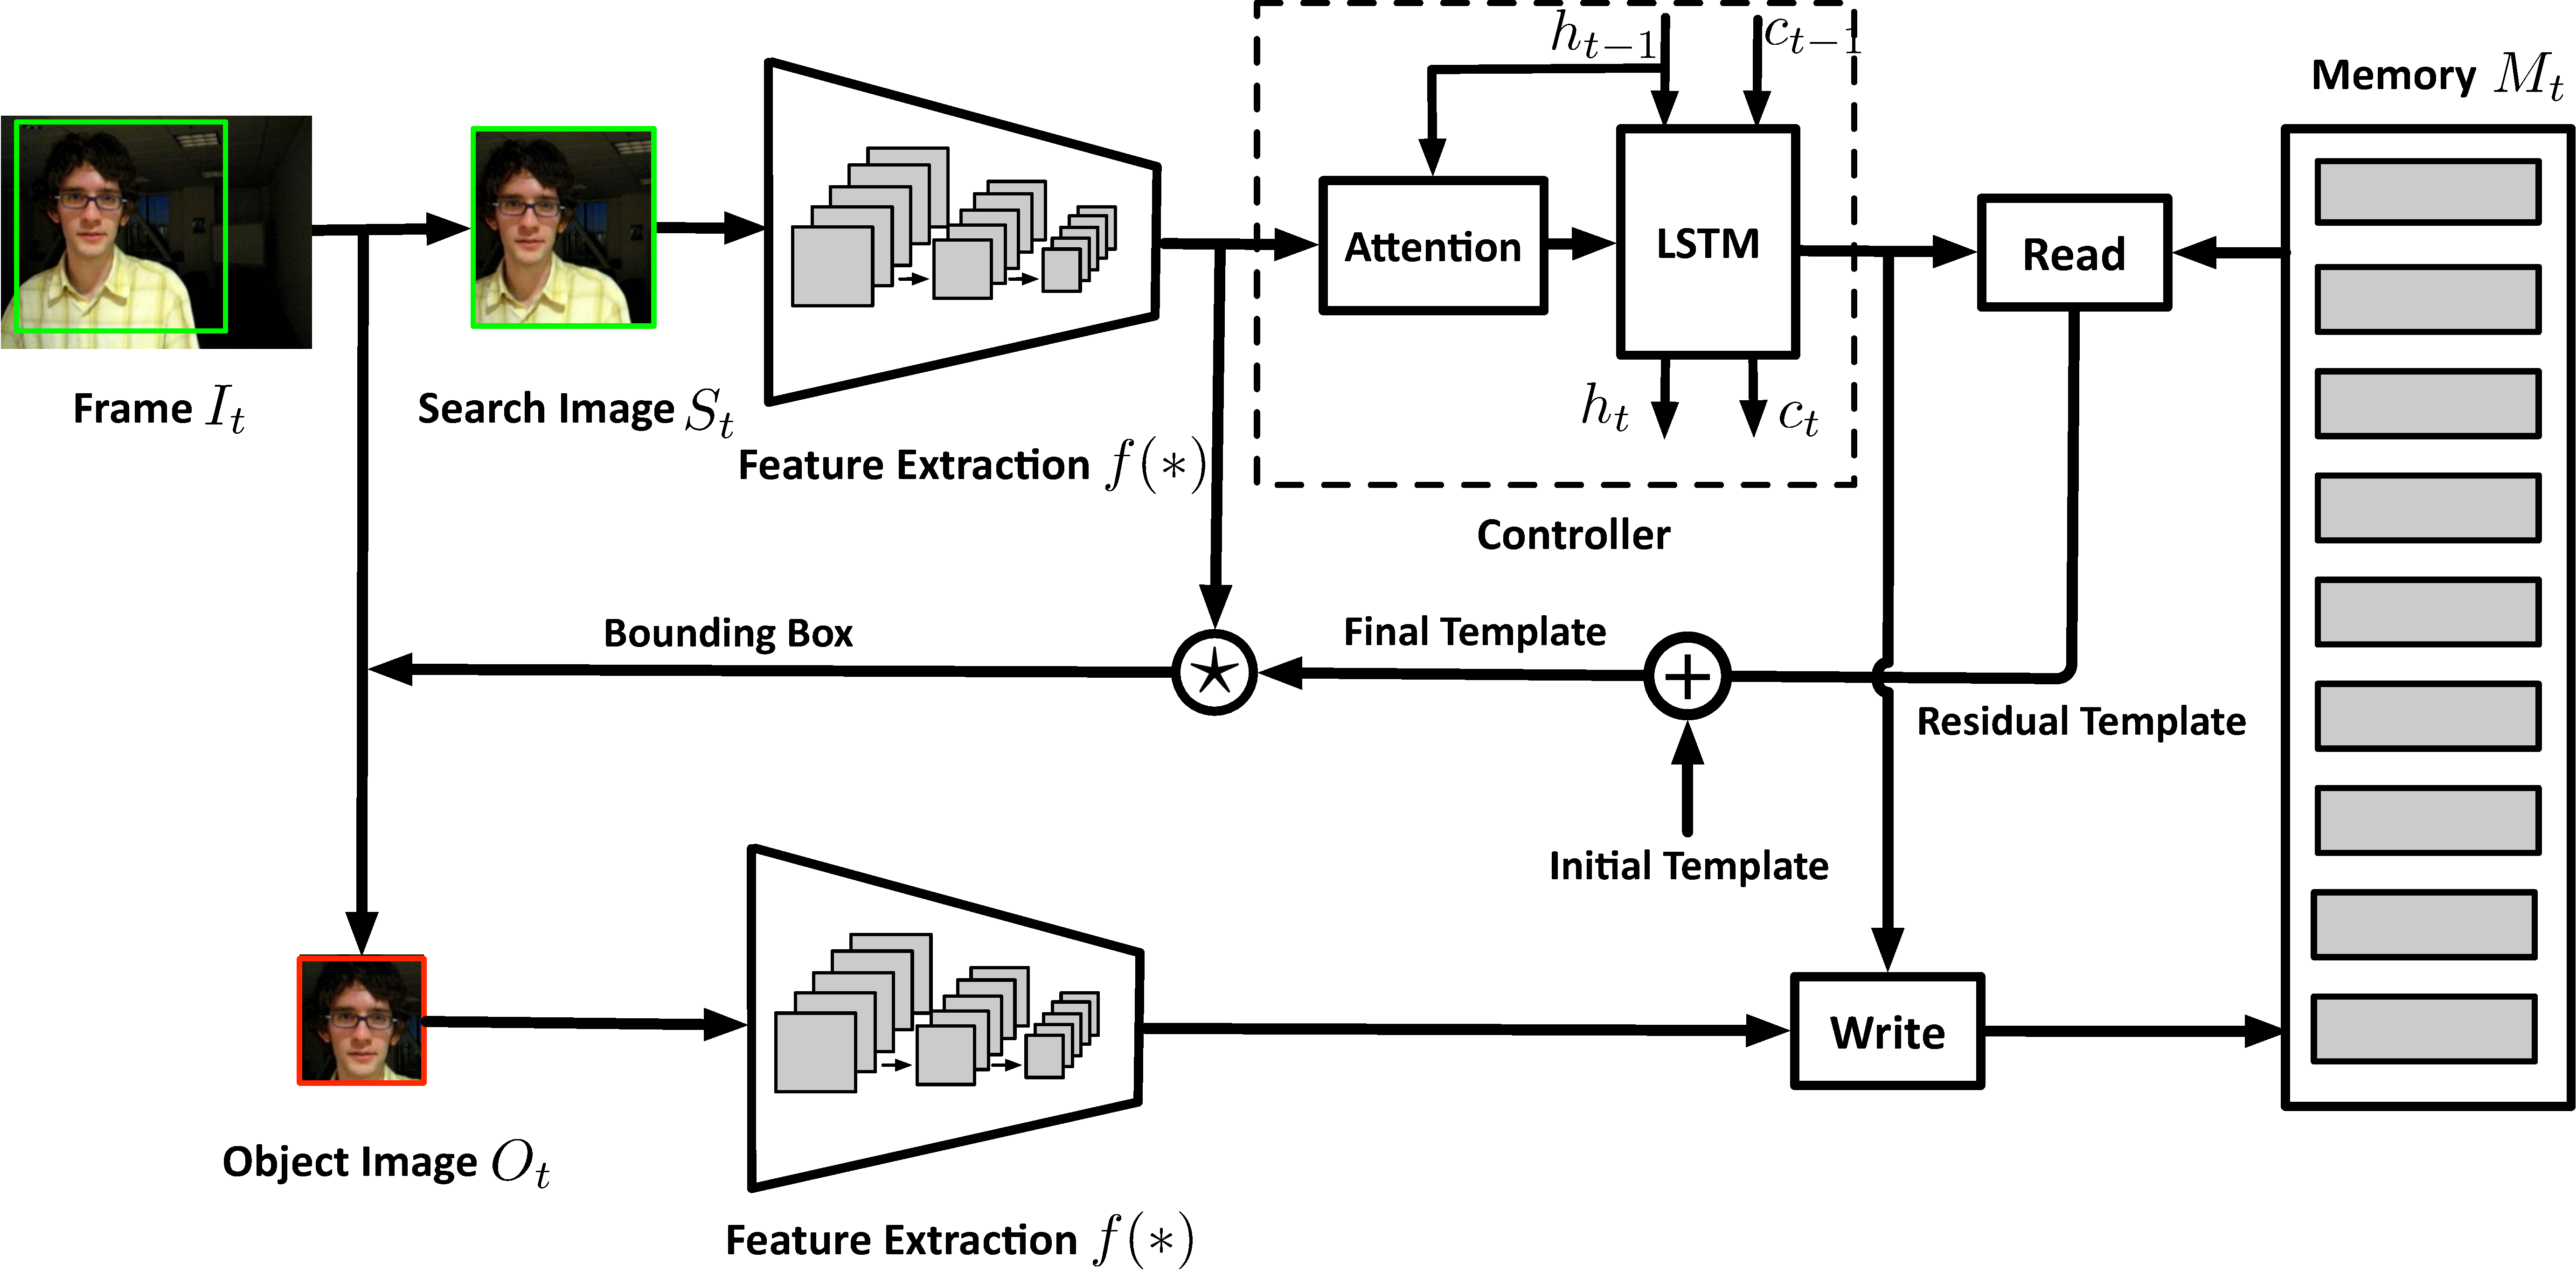
\includegraphics[width=0.95\linewidth]{framework.pdf}
	\end{center}
	\vspace{-3mm}
	\caption{The pipeline of our tracking algorithm. The green rectangle are the candidate region for target searching. The \textit{Feature Extractions} for object image and search image share the same architecture and parameters. An attentional LSTM extracts the target's information on the search feature map, which guides the memory reading process to retrieve a matching template.  The residual  template is combined with the initial template, to obtain a final template for generating the response score. The newly predicted bounding box is then used to crop the object's image patch for memory writing. 
		%	\TODO{add all the variable names for the things, e.g. $h_{t-1}$, $h_t$, $S_t$, etc. Also for other diagrams.}
		%\TODO{remove the red box in the Frame $I_t$ since it's not an input}
	}
	\vspace{-2mm}
	\label{fig:2}
\end{figure*}

In this section we propose a dynamic memory network with reading and writing mechanisms for visual tracking. 
The whole framework is shown in Figure \ref{fig:2}.
Given the search image, first features are extracted with a CNN.
The image features are input into an attentional LSTM, which controls the memory reading and writing. 
A residual templates is read from the memory and combined with the initial template learned from the first frame, forming the final template.  The final template is convolved with the search image features to obtain the response map, and the target bounding box is predicted.
%The final template, which is used for similarity matching, is retrieved from the dynamic memory by a residual template learning process.
The new target's template is cropped using the predicted bounding box, features are extracted and then written into memory for model updating. 

\subsection{Feature Extraction}

Given an input image $I_t$ at time $t$, we first crop the frame into a search image patch $S_t$ with a rectangle that is computed by the previous predicted bounding box. Then it is encoded into a high level representation $f(S_t)$, which is a spatial feature map, via a fully convolutional neural networks (FCNN).  In this work we use the FCNN structure from SiamFC \cite{Bertinetto2016}. 
%\NOTE{is it correct? \yty{there is a minor difference, no group convolution is used, since tensorflow does not support}}
After getting the predicted bounding box, we use the same feature extractor to compute the new object template for memory writing.
%\NOTE{Feature extraction A and B use shared weights? or different weights?  If they are shared, then no need to call it A and B.}

%
%\begin{figure}[t]
%	\begin{center}
%		\includegraphics[width=0.8\linewidth]{figs/att_net.pdf}
%	\end{center}
%	\caption{Diagram of attention network.}
%	\label{fig:3-1}
%\end{figure}

\subsection{Attention Scheme}

%\TODO{insert a sentence about the motivation. Why do we need attention?}
%\TODO{add a figure showing the attention block.}
Since the object information in the search image is needed to retrieve the related template for matching, but the object location is unknown at first, we apply an attention mechanism to make the input of LSTM concentrate more on the target.
We define $\mathbf{f}_{t,i} \in \mathbb{R}^{n \times n \times c}$ as the $i$-th $\mathit{n\times n\times c}$ square patch on $f(S_t)$ in a sliding window fashion.\footnote{We use $6\times6\times256$, which is the same size of the matching template.}
Each square patch covers a certain part of the search image. An attention-based weighted sum of these square patches can be regarded as a soft representation of the object, which can then be fed into LSTM to generate a proper read key for memory retrieval. However the size of this soft feature map is still too large to directly feed into LSTM. 
%
To further reduce the size of each square patch, % for fast retrieval, 
we first adopt an average pooling with $n\times n$ filter size on $f(S_t)$,
\begin{align}
f^*(S_t) = \text{AvgPooling}_{n\times n}(f(S_t))
\end{align}
and $\mathbf{f}^*_{t,i} \in \mathbb{R}^{c}$ is the feature vector %a $c$-dimension vector 
for the $i$th patch. 

The attended feature vector is then computed as the weighted sum of the feature vectors,
%Therefore, the input of LSTM is computed by,
\begin{align}
\mathbf{a}_t = \sum_{i=1}^{L}\alpha_{t,i}\mathbf{f}^*_{t,i}
\end{align}
where $L$ is the number of square patches, and the attention weights $\alpha_{t,i}$ is calculated by a softmax, 
\begin{align}
\alpha_{t,i} = \frac{\exp(r_{t,i})}{\sum_{k=1}^{L}\exp(r_{t,k})}
\end{align}
where 
\begin{align}
r_{t,i} = W^a \text{tanh}(W^h \mathbf{h}_{t-1}+W^f \mathbf{f}^*_{t,i}+b)
\end{align}
is an attention network which takes the previous hidden state $\mathbf{h}_{t-1}$ of the LSTM controller and a square patch $\mathbf{f}^*_{t,i}$ as input. $W^a, W^h, W^f$ and $b$ are weight matrices and biases for the network.

By comparing the target's historical information in the previous hidden state with each square patch, the attention network can generate attentional weights that have higher values on the target and smaller values for surrounding regions.  Figure \ref{fig:3} shows example search images with attention weight maps. We can see that our attention network can always focus on the target which is beneficial when retrieving memory for template matching. 

\begin{figure}[t]
	\begin{center}
		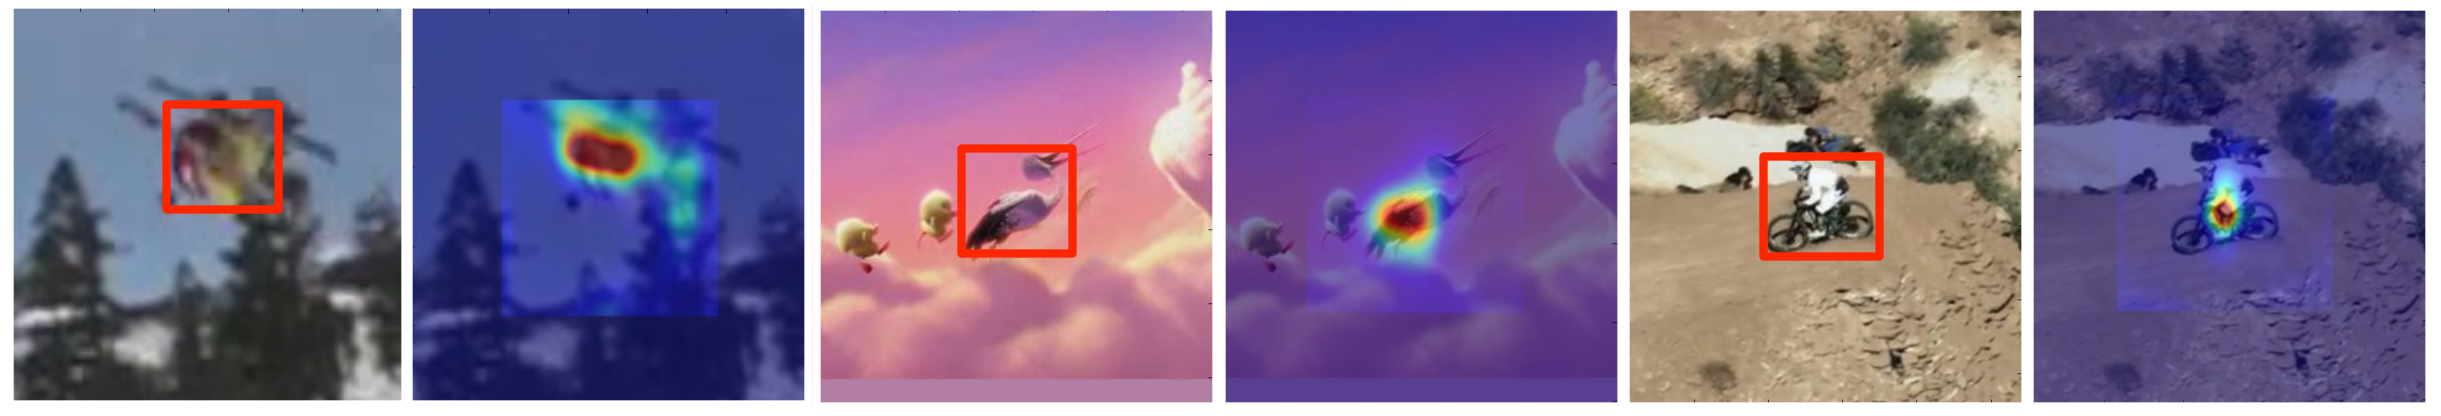
\includegraphics[width=0.9\linewidth]{attention_row.jpg}
	\end{center}
	\vspace{-3mm}
	\caption{Visualization of attentional weights map: \abcn{for each pair, (left) search images and ground-truth target box, and (right) attention maps over search image.}
		For visualization, the attention maps are resized using bicubic interpolation to match the size of the original image.}
	%\TODO{check description.\yty{Since there is no padding when calculating our CNN, area outside this bounding box does not have attention weights. So I just set it zero for clarity. Should I remove this box? \abc{Yes remove box}}} }}
	\vspace{-2mm}
	\label{fig:3}
\end{figure}

\subsection{LSTM Memory Controller}

%\TODO{add some brief info. what is the input/output? output is handled in other sections. anything special?}
For each time step, the LSTM controller takes the attended feature vector $\mathbf{a}_t$, obtained in the attention module, and the previous hidden state $\mathbf{h}_{t-1}$ as input, and outputs the new hidden state $\mathbf{h}_t$ to calculate the memory control signals, including read key, read strength, bias gates, and decay rate (discussed later).
\abcn{The internal architecture of the LSTM uses the standard model (details in the Supplemental), while the output layer is modified to generate the control signals.}
In addition, we also use layer normalization \cite{Ba2016} and dropout regularization \cite{Srivastava2014} for the LSTM. The initial hidden state $\mathbf{h}_0$ and cell state $\mathbf{c}_0$  %\NOTE{check!} 
are  
obtained by passing the initial target's feature map through one $n\times n$ average pooling layer and two separate fully-connected layer with tanh activation functions, respectively.
%constructed by a linear transformation of the initial target's feature map with the tanh activation function.}


\subsection{Memory Reading}
\begin{figure}[t]
	\begin{center}
		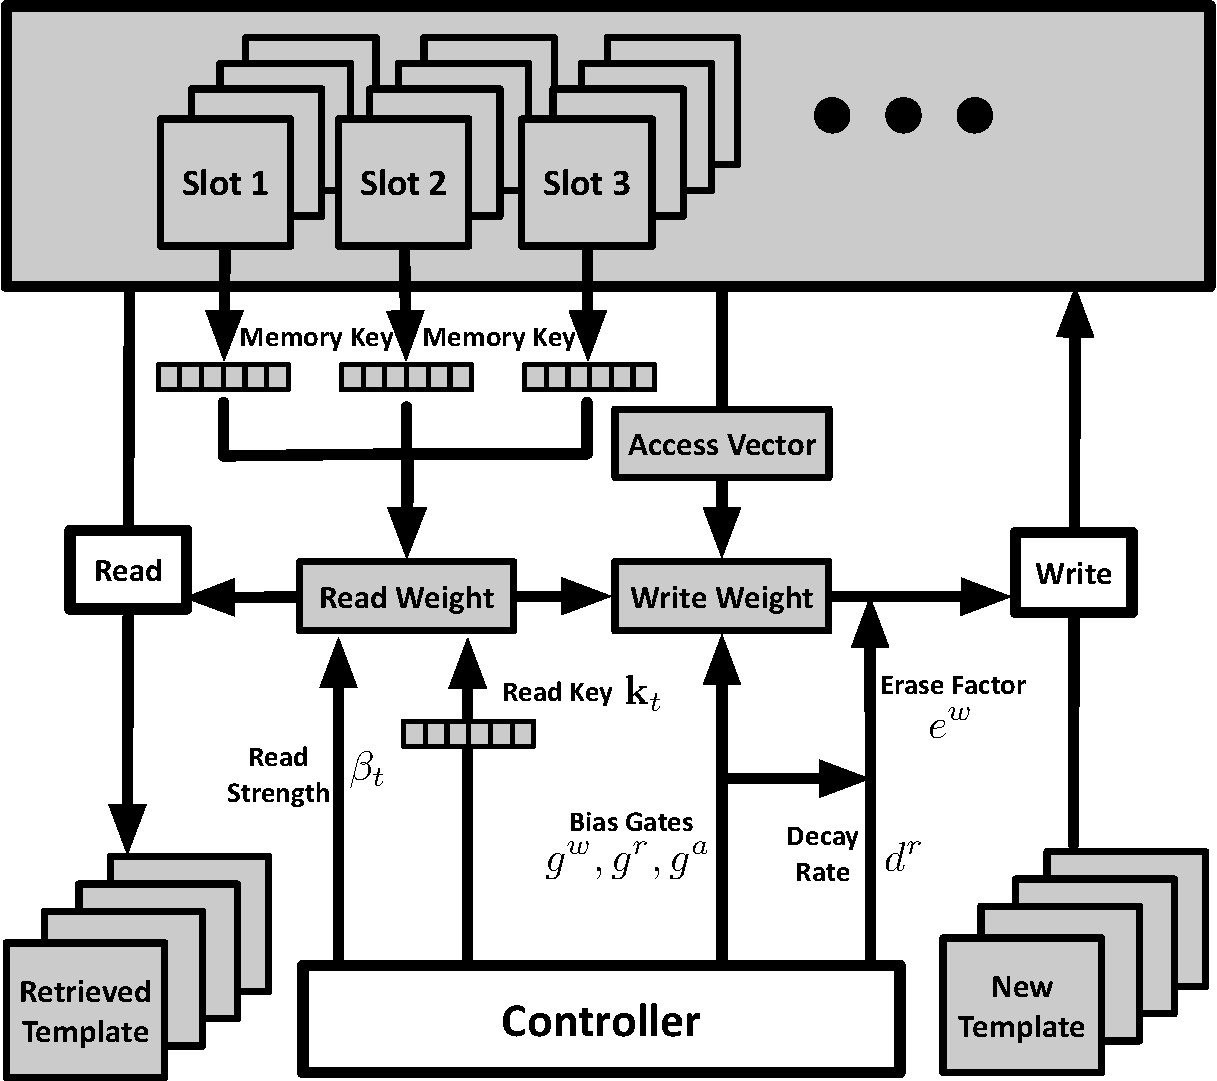
\includegraphics[width=0.61\linewidth]{mem_access.pdf}
	\end{center}
	\vspace{-3mm}
	\caption{Diagram of memory access mechanism.}
	\vspace{-2mm}
	\label{fig:4}
\end{figure}

%\TODO{add a few sentences about the high-level motivation and function.}
Memory is retrieved by computing a weighted summation of all memory slots with a read weight vector, which is determined by the cosine similarity between a read key and the memory keys. This aims at retrieving the most related template stored in memory.
%\NOTE{I changed the index to $j$ so that it isn't confused with $i$ for attention patches.}
Suppose $\mathbf{M}_t \in \mathbb{R}^{N\times n \times n \times c}$ represents the memory module,  such that $\mathbf{M}_t(j) \in \mathbb{R}^{n \times n \times c}$ is the template stored in the $j\text{th}$ memory slot and $N$ is the number of memory slots. 
%
The LSTM controller outputs the read key $\mathbf{k}_t \in \mathbb{R}^{c}$ and read strength $\beta_t \in [1,\infty]$,
\begin{align}
\mathbf{k}_t = & W^k\mathbf{h}_{t}+b^k \\
\beta_t = & 1+\log(1+\exp(W^\beta \mathbf{h}_{t}+b^\beta))
\end{align}
where %$\mathbf{h}_t$ is the hidden state of LSTM and 
$W^k, W^\beta, b^k, b^\beta$ are corresponding weight matrices and biases.
% for linear transformations.
The read key $\mathbf{k}_t$ is used for matching the contents in the memory, while the read strength $\beta_t$ indicates the reliability of the generated read key. 
%
Given the read key and read strength, a \textit{read weight} $\mathbf{w}^r_t\in \mathbb{R}^{N}$ is computed for memory retrieval,
\begin{align}
\mathbf{w}^r_t(j) =\frac{\exp{\{C(\mathbf{k}_t, \mathbf{k}_{\mathbf{M}_t(j)})}\beta_t\}}{\sum_{j'} \exp{\{C(\mathbf{k}_t, \mathbf{k}_{\mathbf{M}_t(j')})}\beta_t\}}
\end{align}
where $\mathbf{k}_{\mathbf{M}_t(j)} \in \mathbb{R}^{c}$ is the memory key generated by a $n\times n$ average pooling on $\mathbf{M}_t(j)$. $C(\mathbf{x}, \mathbf{y})$ is the  cosine similarity between vectors, 
%\begin{align}
$C(\mathbf{x},\mathbf{y})= \frac{\mathbf{x} \cdot \mathbf{y}}{\|\mathbf{x}\|\|\mathbf{y}\|}$.
%\end{align}
Finally, the template is retrieved from memory as a weighted sum,
\begin{align}
\mathbf{T}^{\text{retr}}_t=\sum_{j=1}^N\mathbf{w}^r_t(j)\mathbf{M}_t(j).
\end{align}

\subsection{Residual Template Learning}
%\NOTE{why is it "Learning" the residual?}

Directly using the retrieved template for similarity matching  is prone to overfit recent frames.
Instead, we learn a residual template by multiplying the retrieved template times a channel-wise gate vector and add it to the initial template to capture the appearance changes. Therefore, our final template is formulated as,
\begin{align}
\mathbf{T}^{\text{final}}_t = \mathbf{T}_0+ \mathbf{r}_t\odot \mathbf{T}^{\text{retr}}_t,
\end{align}
where $\mathbf{T}_0$ is the initial template and  $\odot$ is channel-wise multiplication.
%
$\mathbf{r}_t\in \mathbb{R}^c$ is the \textit{residual gate} produced by LSTM controller, 
\begin{align}
\mathbf{r}_t = \sigma (W^r\mathbf{h}_{t}+b^r),
\end{align}
where $W^r, b^r$ are corresponding weights and biases, and $\sigma$ represents sigmoid function. 
%\NOTE{residual vector is not the best name, since it sounds like a residual. It seems more like a weight or a gate.}
The \textit{residual gate} controls how much each channel of the retrieved template is added to the initial one, which can be regarded as a form of feature selection. 

\begin{figure}[t]
	\begin{center}
		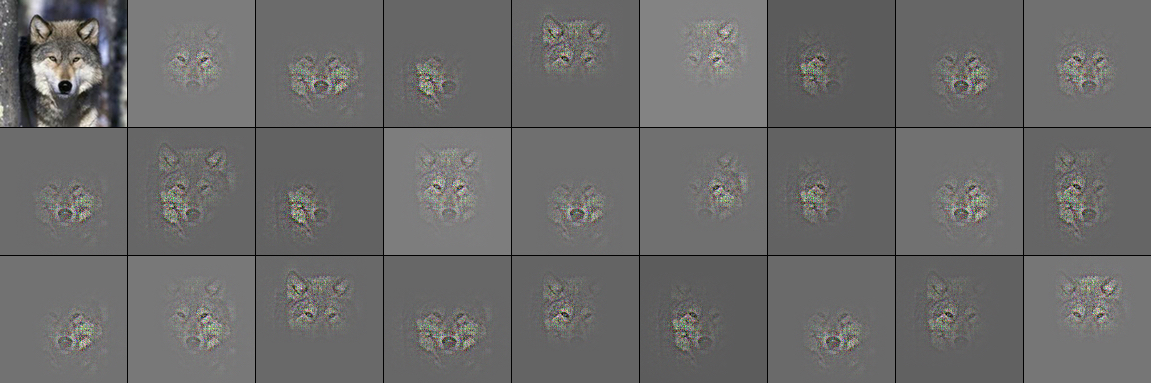
\includegraphics[width=0.65\linewidth]{channel2.jpg}
	\end{center}
	\vspace{-4mm}
	\caption{The feature channels respond to target parts: images are reconstructed from conv5 of the CNN used in our tracker. Each image is generated by accumulating reconstructed pixels from the same channel. The input image is shown in the top-left. }
	\vspace{-2mm}
	\label{fig:6}
\end{figure}

By projecting different channels of a target feature map to pixel-space using deconvolution, as in \cite{Zeiler2014}, we find that the channels focus on different object parts (see Figure \ref{fig:6}). % \TODO{missing figure}). 
Thus, the channel-wise feature residual learning has the advantage of updating different object parts separately. Experiments in Section \ref{abla} show that this yields a big performance improvement. 

%\TODO{how to get the response map? How to get the predicted bounding box?\yty{in Implementation details.}}

\subsection{Memory Writing}

The image patch with the new position of the target is used for model updating, \emph{i.e.}, memory writing.
%As is shown in Figure \ref{fig:2}, we extract the object patch with the new position of target for model updating, \emph{i.e.}, memory writing. 
The new object template $\mathbf{T}^{\text{new}}_t$ is computed using the feature extraction CNN. There are three cases for memory writing: 1) when the new object template is not reliable (e.g.\ contains a lot of background), there is no need to write new information into memory; 2) when the new object appearance does not change much compared with the previous frame, the memory slot that was previously read should be updated; %we should just follow the read position for memory updating;
3) when the new target has a large appearance change, a new memory slot should be overwritten.
%we would like this information to be written into a new position of memory module. Thereby, 
To handle these three cases, we define the \textit{write weight} as
\begin{align}
\mathbf{w}^w_t =g^w\mathbf{0}+g^r\mathbf{w}^r_t + g^a\mathbf{w}^a_t, 
\end{align}
where $\mathbf{0}$ is the zero vector, $\mathbf{w}^r_t$ is the read weight, and $\mathbf{w}^a_t$  is the allocation weight, which is responsible for allocating a new position for memory writing. 
The write gate $g^w$, read gate $g^r$ and allocation gate $g^a$, are produced by the LSTM controller with a softmax function, 
\begin{align}
[g^w, g^r, g^a] = \text{softmax}(W^g \mathbf{h}_{t}+b^g),
\end{align}
where $W^g, b^g$ are the weights and biases. Since $g^w+g^r+g^a=1$, these three gates govern the interpolation between the three cases.  If $g^w=1$, then $\mathbf{w}^w_t=\mathbf{0}$ and nothing is written.  If $g^r$ or $g^a$ have higher value, then the new template is either used to update the old template (using $\mathbf{w}^r_t$) or written into newly allocated position (using $\mathbf{w}^a_t$). The \textit{allocation weight} is calculated by,
\begin{align}
\mathbf{w}^a_t(i)=
\begin{cases}
1, &\text{if } i=\displaystyle \mathop{\mathrm{argmin}}_{i} \mathbf{w}^u_{t-1}(i)\\
0, &\text{otherwise}
\end{cases}
\end{align}
where $\mathbf{w}^u_t$ is the \textit{access vector},
\begin{align}
\mathbf{w}^u_t = \lambda \mathbf{w}^u_{t-1} + \mathbf{w}^r_t + \mathbf{w}^w_t,
\end{align}
which indicates the frequency of memory access (both reading and writing), and $\lambda$ is a decay factor. Memory slots that are accessed infrequently will be assigned new templates.  
%\TODO{what is $\lambda$? is it learned?}

The writing process is performed with a \textit{write weight} in conjunction with an \textit{erase factor} for clearing the memory, 
\begin{align}
\mathbf{M}_{t+1}(i) = \mathbf{M}_{t}(i)(\mathbf{1}-\mathbf{w}^w_t(i)e^w)+\mathbf{w}_t(i)^we^w\mathbf{T}^{\text{new}}_t,
\end{align}
where %$\mathbf{T}^{\text{new}}_t$ is the new target template and
$e^w$ is the \textit{erase factor} computed by
\begin{align}
e^w = d^rg^r+g^a,
\end{align}
and $d^r \in [0,1]$ is the \textit{decay rate} produced by the LSTM controller, 
\begin{align}
d^r = \sigma (W^d\mathbf{h}_{t}+b^d),
\end{align}
where $\sigma$ is sigmoid function. $W^d$ and $b^d$ are corresponding weights and biases. If $g^r=1$ (and thus $g^a=0$), then $d^r$ serves as the decay rate for updating the template in the memory slot (case 2). If $g^a=1$ (and $g^r=0$), $d^r$ has no effect on $e^w$, and thus the memory slot will be erased before writing the new template (case 3). Figure \ref{fig:4} shows the detailed diagram of the memory reading and writing process.

\section{Implementation Details}
We adopt an Alex-like CNN as in SiamFC \cite{Bertinetto2016} for feature extraction, where the input image sizes of the object  and search images are $127\times 127 \times 3$ and $255 \times 255 \times 3$ respectively. The whole network is trained offline on the VID dataset (object detection from video) of ILSVRC \cite{ILSVRC15} from scratch, and takes about a day. %\yty{It takes about a day to train the whole network.}  
Adam \cite{kingma2014adam} optimization is used with a mini-batches of 8 video clips of length 16. The initial learning rate is 1e-4 and is multiplied by 0.8 every 10k iterations. The video clip is constructed by %randomly and 
uniformly sampling frames \abc{(keeping the temporal order)} from each video. \ytyy{This aims to diversify the appearance variations in one episode for training, which can simulate fast motion, fast background change, jittering object, low frame rate.}
We use data augmentation, including small image stretch and translation for the target image and search image. 
The dimension of memory states in the LSTM controller is 512 and the retain probability used in dropout for LSTM is 0.8. The number of memory slots is $N=8$. The decay factor used for calculating the access vector is $\lambda=0.99$.
%
%\TODO{any other parameters? $\lambda$?}
%\TODO{what is the offline training time?}
At test time, the tracker runs completely feed-forward and no online fine-tuning is needed. We locate the target based on the upsampled response map as in SiamFC \cite{Bertinetto2016}, and handle the scale changes by searching for the target over three scales $1.05^{[-1,0,1]}$. To smoothen scale estimation and penalize large displacements, we update the object scale with the new one by a decay rate 0.6 and dampen the response map with a cosine window by decay rate 0.15.
%\TODO{anything to say about the tracking process?}
%\TODO{how to get the target scale?}

Our algorithm is implemented in Python with the TensorFlow toolbox \cite{abadi2016tensorflow}. It runs at about 50 fps on a computer with four Intel(R) Core(TM) i7-7700 CPU @ 3.60GHz and a single NVIDIA GTX 1080 Ti with 11GB RAM.


\section{Experiments}

We evaluate our proposed tracker, denoted as MemTrack, on three challenging datasets: OTB-2013 \cite{Wu2013}, OTB-2015 \cite{Wu2015} and VOT-2016 \cite{Kristan2016}.  We follow the standard protocols, and evaluate using precision and success plots, as well as area-under-the-curve (AUC).

\subsection{Ablation Studies}\label{abla}


\begin{figure}[t]
	\begin{center}
		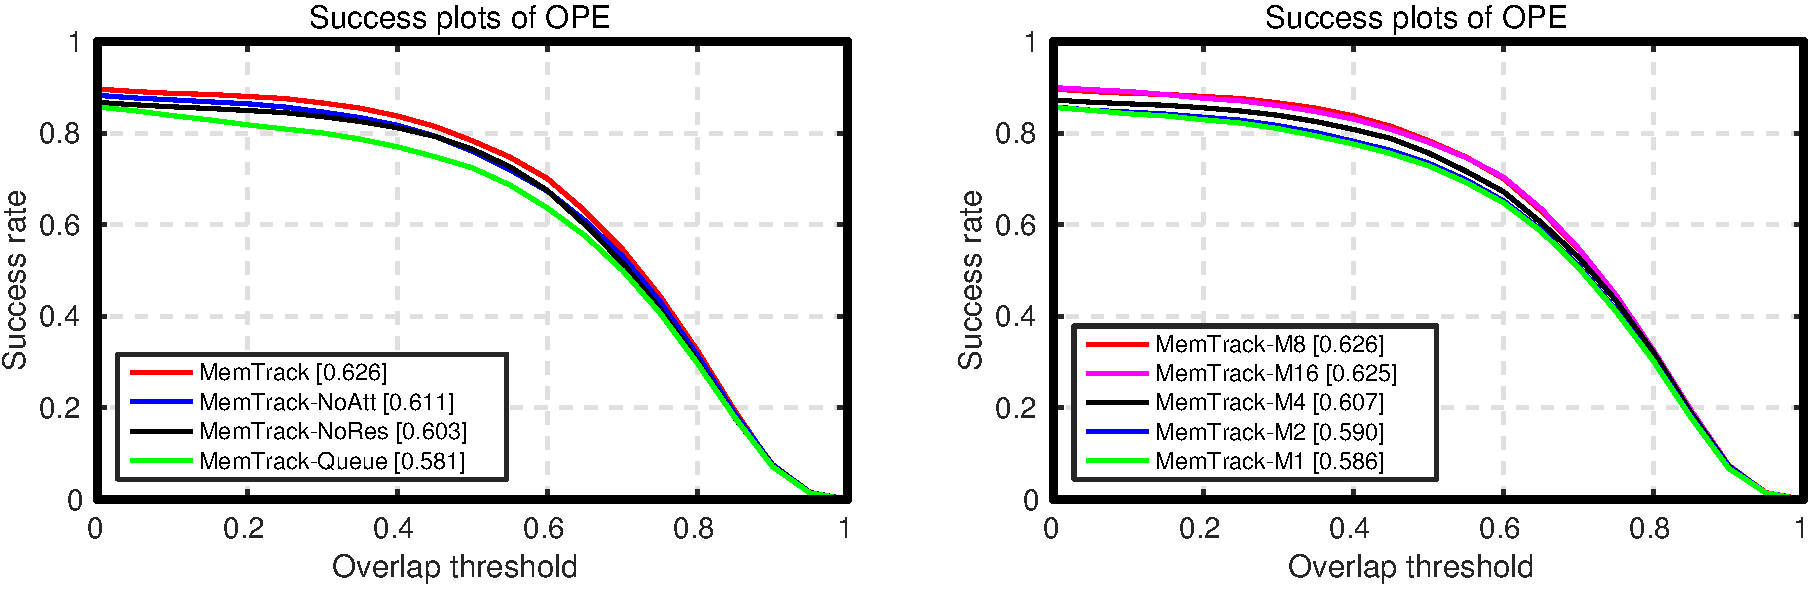
\includegraphics[width=0.85\linewidth]{ablation-tb100.pdf}
	\end{center}
	\vspace{-5mm}
	\caption{Ablation studies: (left) success plots of different variants of our tracker on OTB-2015; (right) success plots for different memory sizes \{1, 2, 4, 8, 16\} on OTB-2015. 
		% \NOTE{Why the right plot so noisy? Maybe some unlucky trials.  How about just plotting N=1, 2, 4, 8, 16.}
	}
	\vspace{-2mm}
	\label{fig:7}
\end{figure}

Our \abc{MemTrack} tracker contains \abc{three important components:} 1) an attention mechanism, which calculates the attended feature vector for memory reading; 2) a dynamic memory network, which maintains the target's appearance variations; and 3) residual template learning, which controls the amount of model updating \abc{for each channel of the template}. To evaluate their separate contributions to our tracker, we implement several variants of our method and verify them on OTB-2015 dataset. 

\yty{ We first design a variant of MemTrack without attention mechanism (MemTrack-NoAtt), which averages all $L$ feature vectors to get the %attended 
feature vector $\mathbf{a}_t$ \abcn{for the LSTM input.} 
Mathematically, it changes %Equation 
(2) to $\mathbf{a}_t = \frac{1}{L}\sum_{i=1}^{L}\mathbf{f}^*_{t,i} $. As we can see in Figure \ref{fig:7} (left), Memtrack without attention decreases performance, \abc{which shows the benefit of using attention to roughly localize the target in the search image.}} 
We also design a naive strategy that simply writes the new target template sequentially into the memory slots as a queue (MemTrack-Queue). When the memory is fully occupied, the oldest template will be replaced with the new  template. The retrieved template is generated by averaging all templates stored in the memory slots. As seen in Fig.~\ref{fig:7} (left), such simple approach cannot produce good performance, \abc{which shows the necessity of our dynamic memory network}. 
\yty{To verify the effectiveness of \abc{gated} residual template learning, we design another variant of MemTrack--- removing channel-wise residual gates (MemTrack-NoRes), \emph{i.e.} directly adding the retrieved and initial templates to get the final template. From Fig.~\ref{fig:7} (left), our \abc{gated} residual template learning mechanism boosts the performance as it helps to select correct residual channel features for template updating.}

We also investigate the effect of memory size  on tracking performance. Figure \ref{fig:7} (right) shows success plots on OTB-2015 using different numbers of memory slots. Tracking accuracy increases along with the memory size and saturates at 8 memory slots. Considering the runtime and memory usage, we choose 8 as the default number. %need more analysis later
%\TODO{more analysis}

\subsection{Comparison Results}

We compare our method MemTrack with 9 recent {\em real-time} trackers ($\geq$ 15 fps), including CFNet \cite{Valmadre2017}, LMCF \cite{Wang2017}, ACFN \cite{Choi2017}, RFL \cite{Yang2017}, SiamFC \cite{Bertinetto2016}, SiamFC\_U \cite{Valmadre2017}, Staple \cite{Bertinetto2016-1}, DSST \cite{Danelljan2014}, and KCF \cite{Henriques2015} on both OTB-2013 and OTB-2015. 
%\NOTE{all of these are template trackers? \yty{RFL, SiamFC, SiamFC\_U are template based trackers, all others are Correlation Filter based ones. CFNet incorporates correlation filter into Siamese network.}}
To further show our tracking accuracy, we also compared with another 8 recent state-of-the art trackers that are {\em not} real-time speed, including CREST \cite{Song2017},  CSR-DCF \cite{Lukezic2017}, MCPF \cite{Zhang2017}, SRDCFdecon \cite{Danelljan2016}, SINT \cite{Tao2016}, SRDCF \cite{Danelljan2015}, HDT \cite{Qi2016}, HCF \cite{Ma2015} on OTB-2015.
%\NOTE{all of these are tracking-by-detection? or do fine-tuning? \yty{CREST, HDT, HCF are trackign by detection, MCPF, SRDCFdecon, SRDCF are Correlation Filter Based, SINT is matching based.}}

\begin{figure}[t]
	\begin{center}
		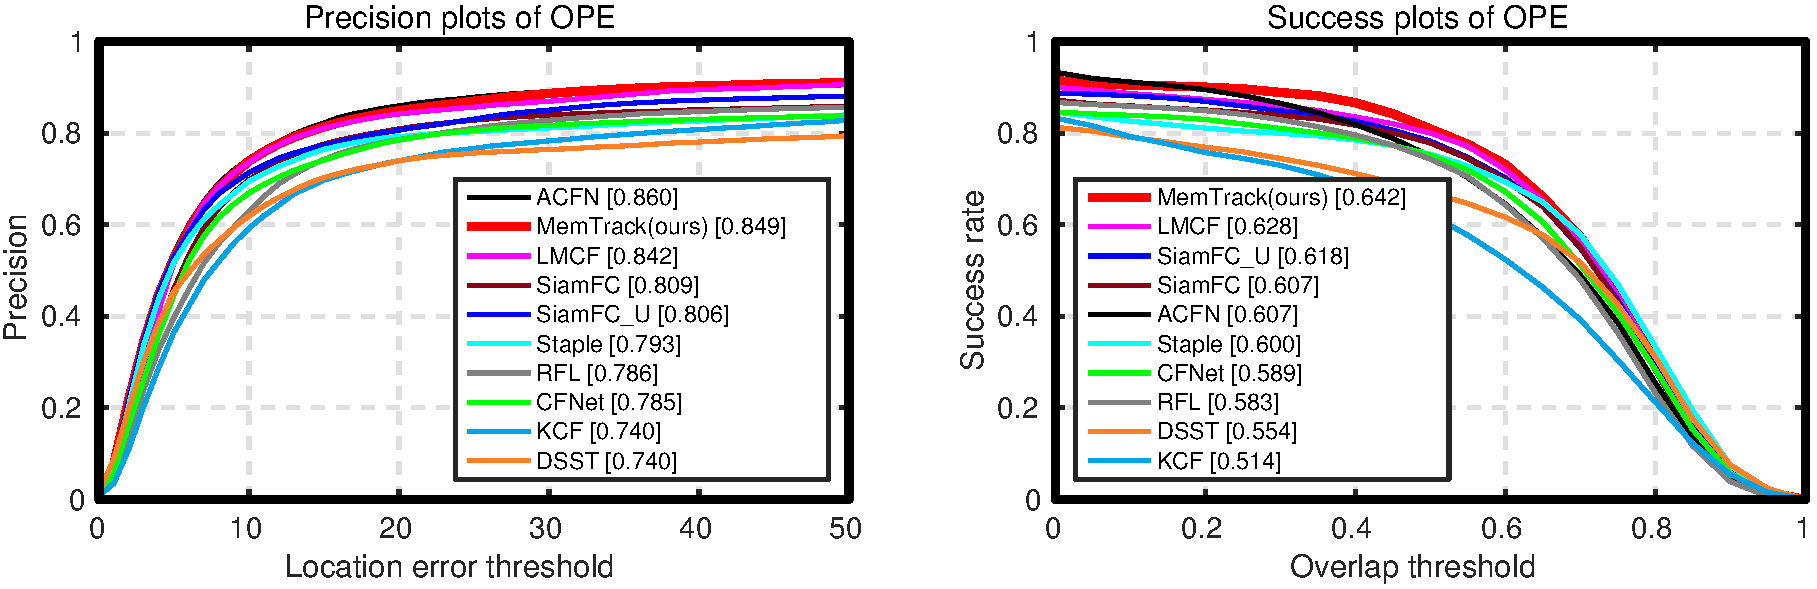
\includegraphics[width=0.85\linewidth]{realtime-cvpr13.pdf}
	\end{center}
	\vspace{-5mm}
	\caption{Precision and success plot on OTB-2013 for recent real-time trackers.
		%		\NOTE{hard to tell what is going on. Make the other lines thinner (and ours thicker). Also put "(ours)" after MemTrack.  Also for other figures.}
	}
	\label{fig:8}
\end{figure}

\textbf{OTB-2013 Results:} OTB-2013 \cite{Wu2013} dataset contains 51 sequences with 11 video attributes and two evaluation metrics, which are center location error and overlap ratio. Figure \ref{fig:8} shows the one-pass comparison results with recent real-time trackers on OTB-2013. Our tracker achieves the best AUC on the success plot and second place on precision plot. Compared with SiamFC \cite{Bertinetto2016}, which is the baseline for matching-based methods without online updating, our tracker 
achieves an improvement of 4.9\% on precision plot and 5.8\% on success plot.
% \NOTE{actually this is absolute increase, not the percentage.  The percentage increase for success plot is (642-607)/607 = 5.7\%}. 
Our method also outperforms SiamFC\_U, the improved version of SiamFC \cite{Valmadre2017} that uses simple linear interpolation of the old and new filters with a small learning rate for online updating. 
This indicates that our dynamic memory networks can handle object appearance changes better than simply interpolating new templates with old ones.


\begin{figure}[t]
	\begin{center}
		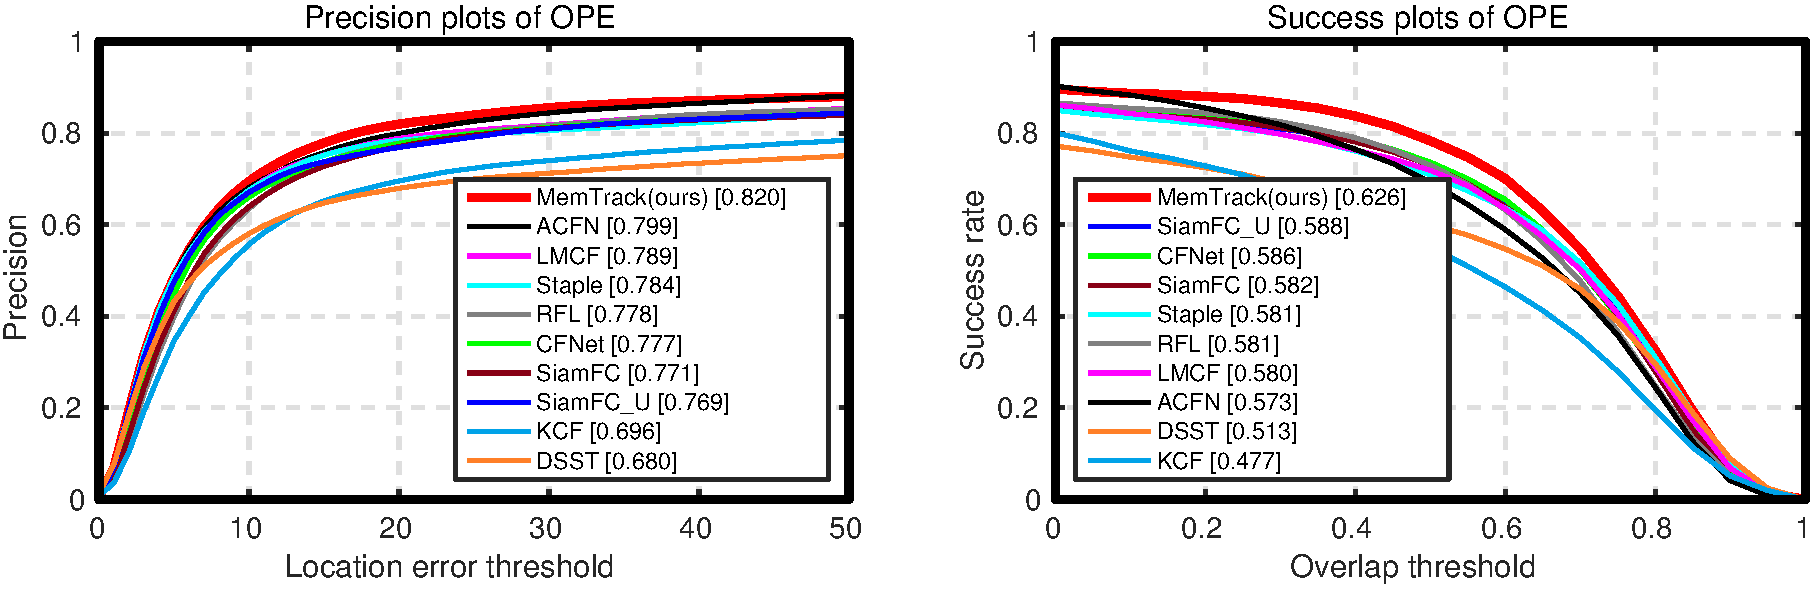
\includegraphics[width=0.85\linewidth]{realtime-tb100.pdf}
	\end{center}
	\vspace{-5mm}
	\caption{Precision and success plot on OTB-2015 for recent real-time trackers.}
	\label{fig:9}
\end{figure}

\textbf{OTB-2015 Results:} The OTB-2015 \cite{Wu2015} dataset is the extension of OTB-2013 to 100 sequences, and is thus more challenging.
%.  It includes 100 sequences, thus is more challenging. 
Figure \ref{fig:9} presents the precision plot and success plot for recent real-time trackers. Our tracker outperforms all other methods in both measures. Specifically, our method performs much better than RFL \cite{Yang2017}, which uses the memory states of LSTM to maintain the object appearance variations. This demonstrates the effectiveness of using an external addressable memory to manage object appearance changes, compared with using LSTM memory which is limited by the size of the hidden states.
% \NOTE{not network parameters...it should be the hidden/cell state size}. 
Furthermore, MemTrack improves the baseline of template-based method SiamFC \cite{Bertinetto2016} with 6.4\% on precision plot and 7.6\% on success plot respectively. % \NOTE{same comment about percentages}. 
Our tracker also outperforms the most recently proposed two trackers, LMCF \cite{Wang2017} and ACFN \cite{Choi2017}, on AUC score with a large margin.
\begin{figure}[t]
	\begin{center}
		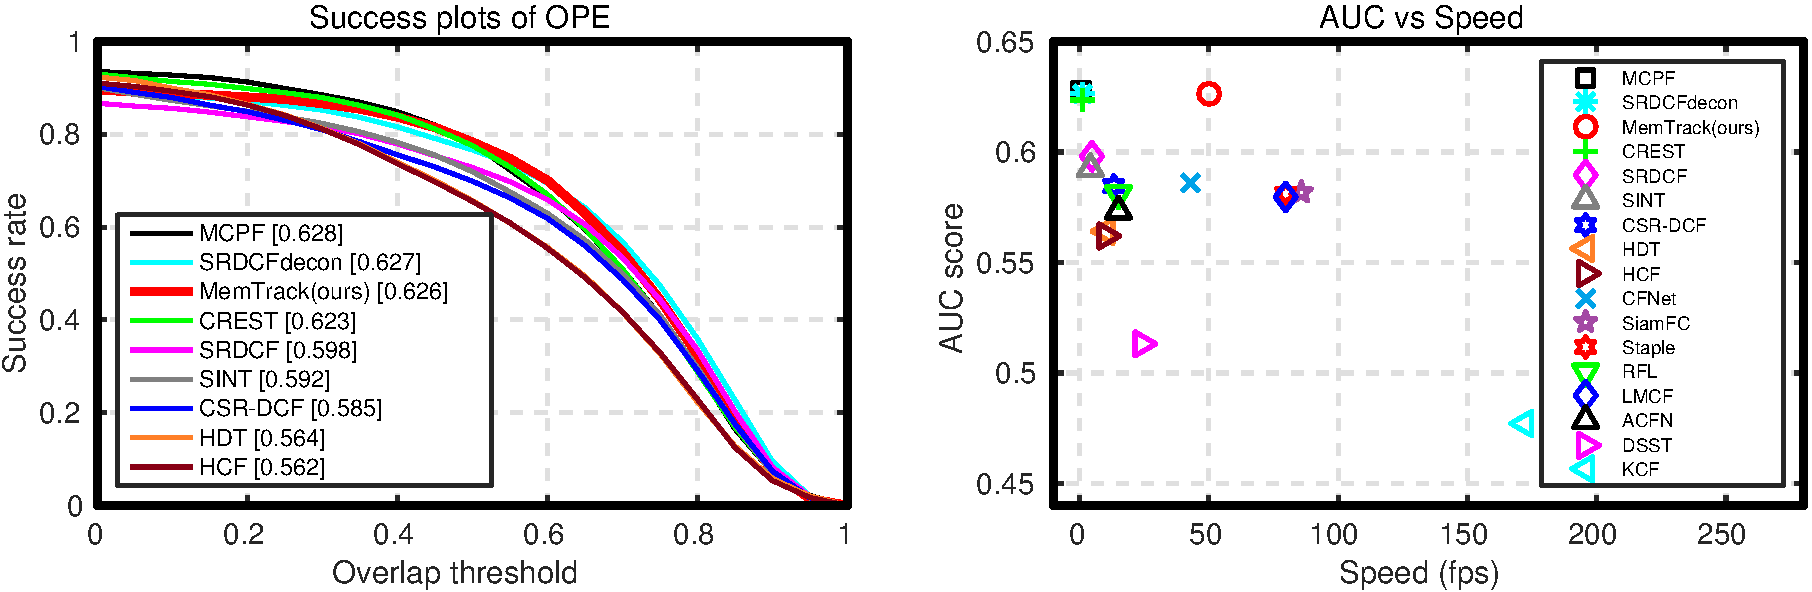
\includegraphics[width=0.85\linewidth]{slow-tb100.pdf}
	\end{center}
	\vspace{-5mm}
	\caption{(left) Success plot on OTB-2015 comparing our real-time MemTrack with recent {\em non-real-time} trackers. (right) AUC score vs speed with recent trackers.}
	\label{fig:10}
\end{figure}
Figure \ref{fig:10} presents the comparison results of 8 recent state-of-the-art {\em non-real time} trackers for AUC score (left plot), and the AUC score vs speed (right plot) of all trackers.
Our MemTrack, which runs in real-time, has similar AUC performance to CREST \cite{Song2017}, MCPF \cite{Zhang2017} and SRDCFdecon \cite{Danelljan2016}, which all run at about 1 fps.
% have similar performance with our tracker but can only run at about 1 fp
%Our MemTrack can perform favorably against them, while running much faster than other methods. Specifically, CREST \cite{Song2017}, MCPF \cite{Zhang2017} and SRDCFdecon \cite{Danelljan2016} have similar performance with our tracker but can only run at about 1 fps. 
Moreover, our MemTrack also surpasses SINT, which is another matching-based method with optical flow as motion information, in terms of both accuracy and speed.
\begin{figure*}[t]
	\begin{center}
		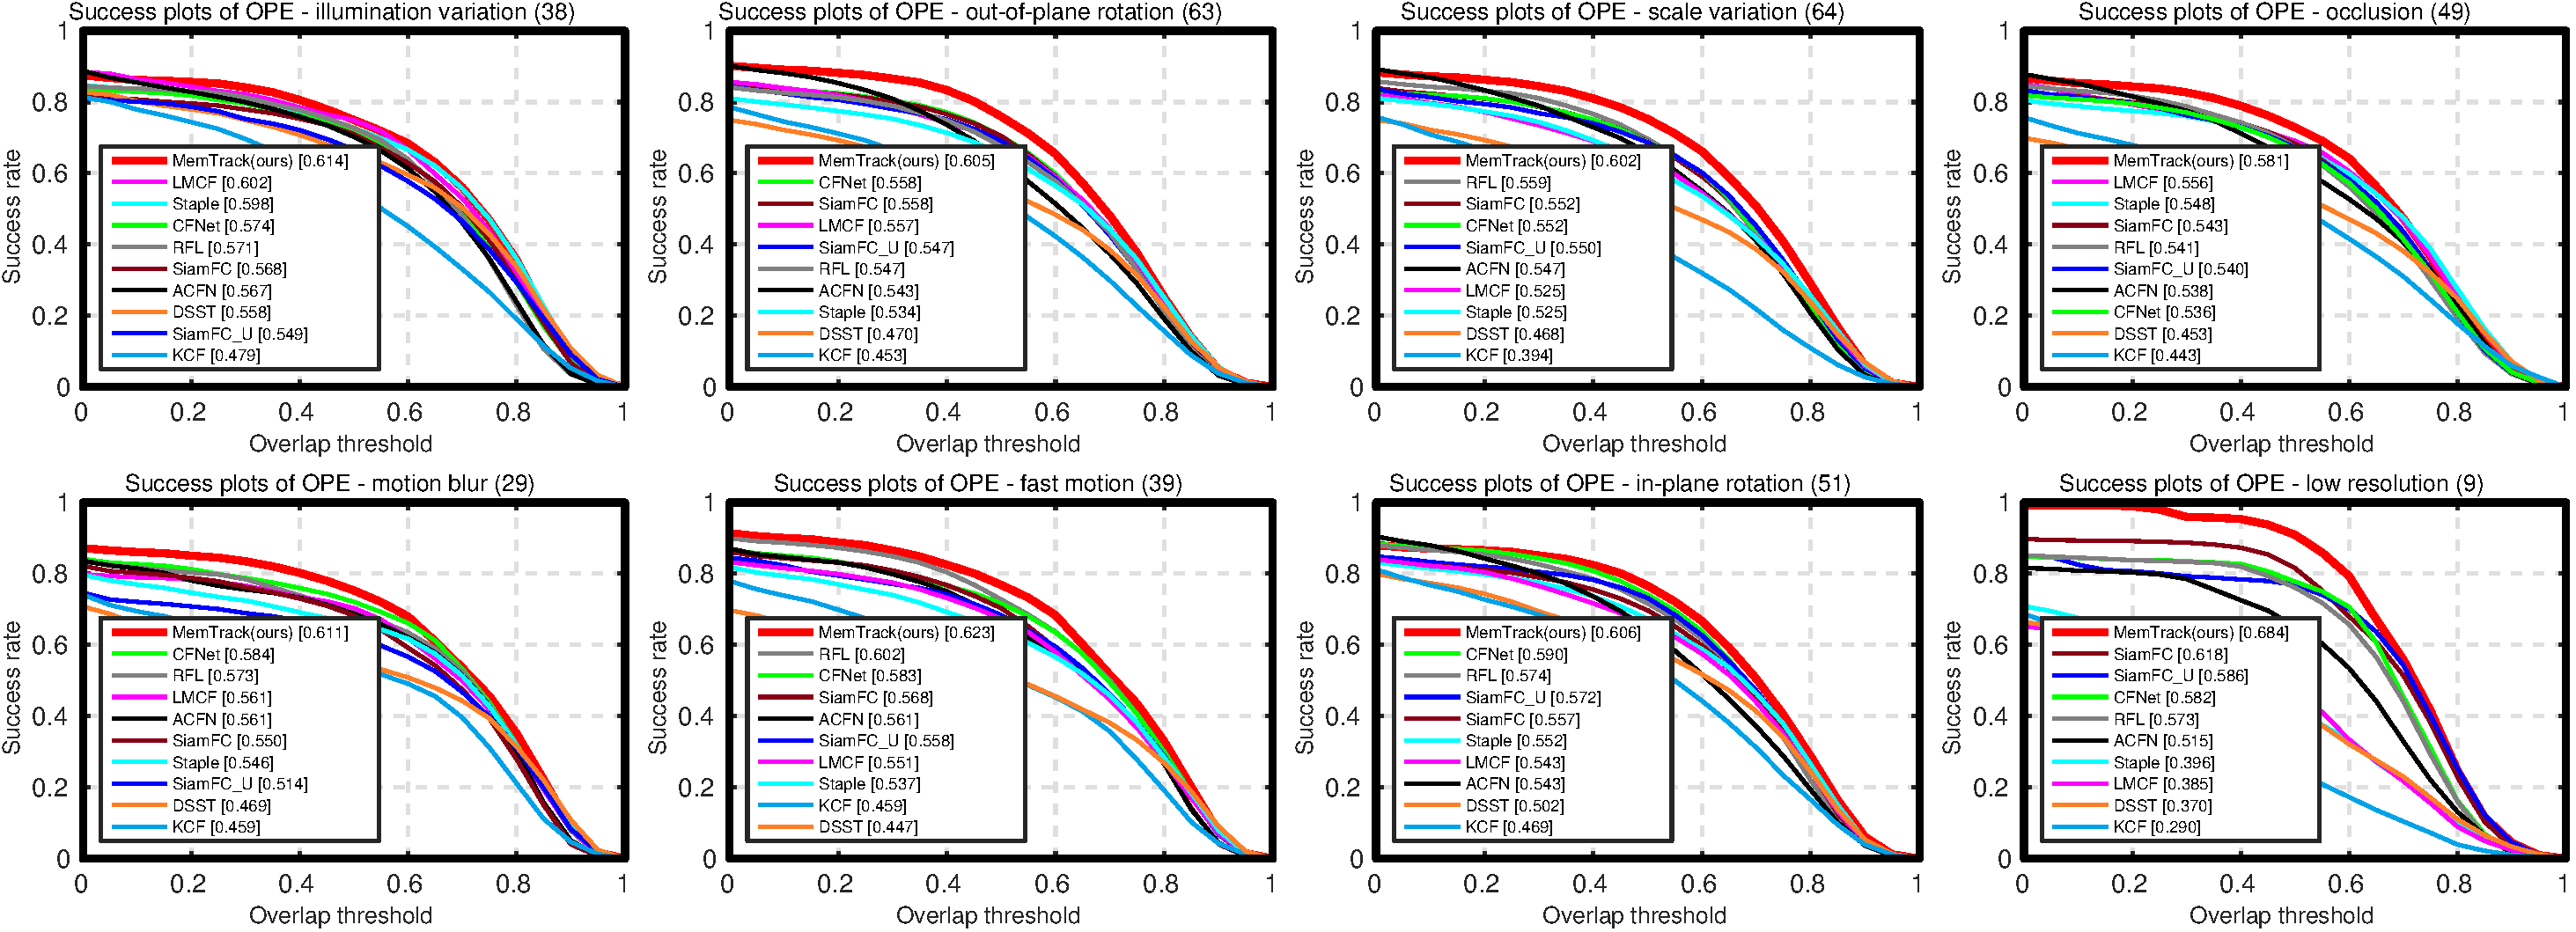
\includegraphics[width=\linewidth]{realtime-attri-tb100.pdf}
	\end{center}
	\vspace{-5mm}
	\caption{The success plot of OTB-2015 on eight challenging attributes: illumination variation, out-of-plane rotation, scale variation, occlusion, motion blur, fast motion, in-plane rotation and low resolution }
	\label{fig:11}
\end{figure*}
Figure \ref{fig:11} further shows the AUC scores of real-time trackers on OTB-2015 under different video attributes including illumination variation, out-of-plane rotation, scale variation, occlusion, motion blur, fast motion, in-plane rotation, and low resolution. Our tracker outperforms all other trackers on these attributes. In particular, for the low-resolution attribute, our MemTrack surpasses the second place (SiamFC) with a 10.7\% improvement on AUC score. % \NOTE{same comment about percentages}. 
In addition, our tracker also works well under out-of-plane rotation and scale variation.
%\NOTE{what about the other 3 attributes? \yty{second palce for background clutter and deformation, first place for out-of-view}}. 
Fig.~\ref{fig:12} shows some qualitative results of our tracker compared with 6 real-time trackers. 

%some qualitative examples
%\TODO{add some qualitative examples}

\begin{figure*}[t]
	\begin{center}
		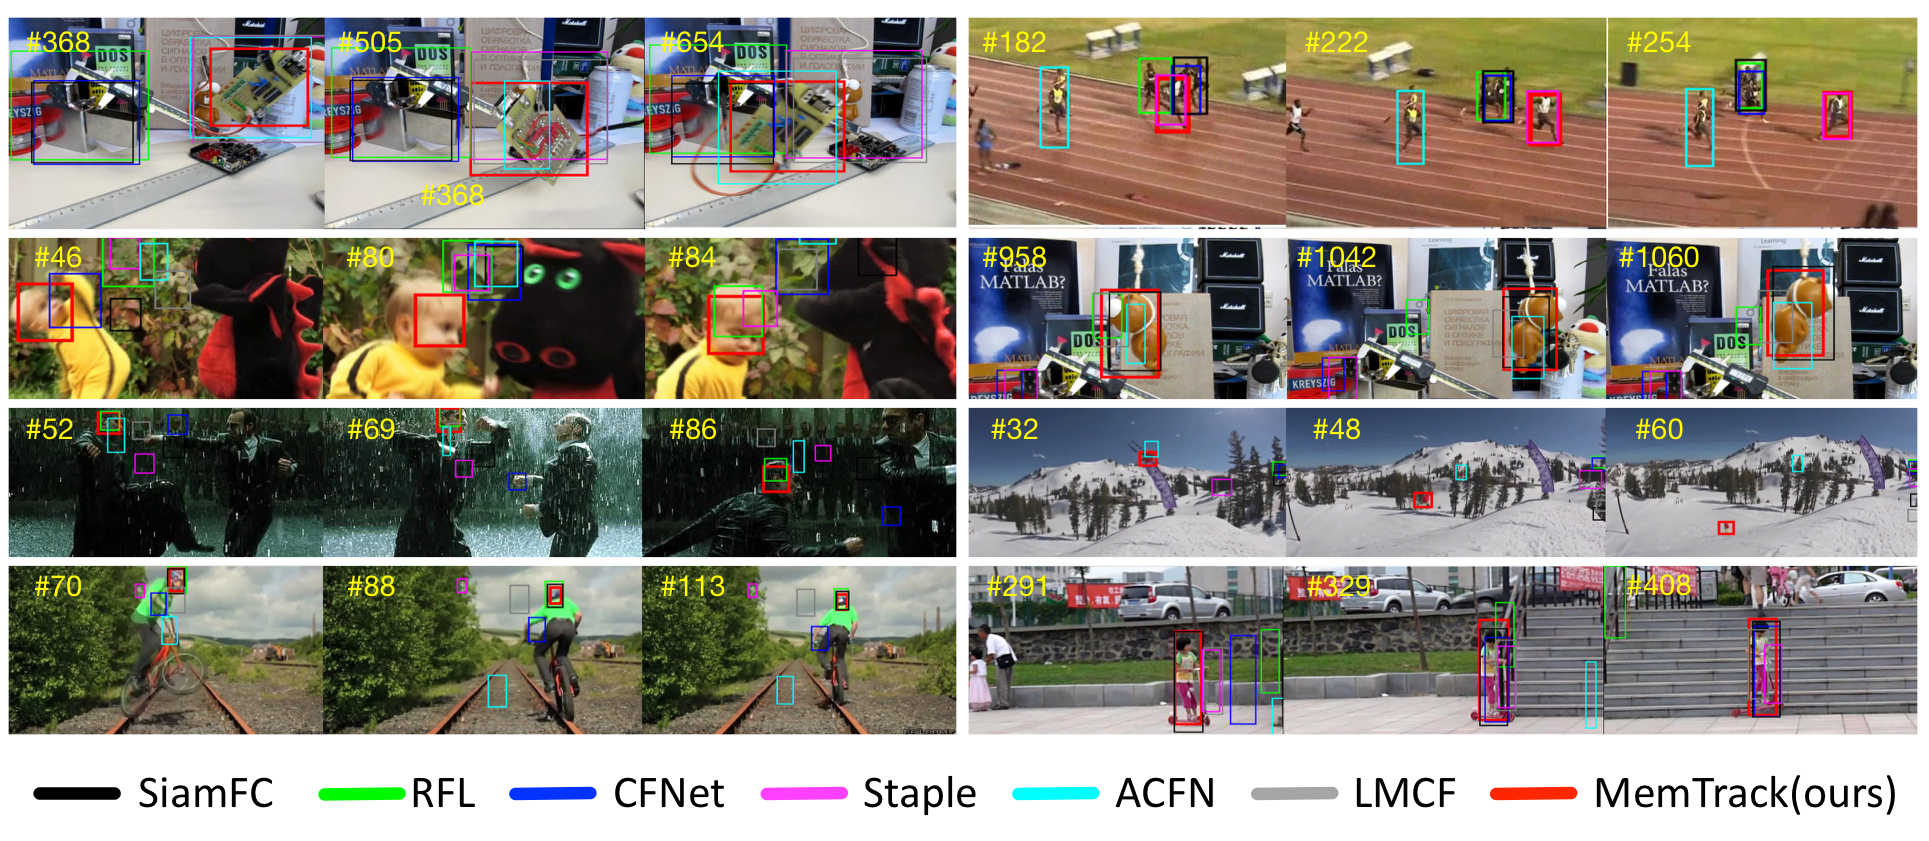
\includegraphics[width=0.95\linewidth]{qualitative.jpg}
	\end{center}
	\vspace{-5mm}
	\caption{Qualitative results of our MemTrack, along with  SiamFC \cite{Bertinetto2016}, RFL \cite{Yang2017}, CFNet \cite{Valmadre2017},  Staple \cite{Bertinetto2016-1}, LMCF \cite{Wang2017}, ACFN \cite{Choi2017} on eight challenge sequences. From left to right, top to bottom: \textit{board, bolt2, dragonbaby, lemming, matrix, skiing, biker, girl2}.}
	\label{fig:12}
\end{figure*}

\begin{table*}
	\small
	\begin{center}
		\bgroup
		\def\arraystretch{1.15}
		\begin{tabular}{ccccccccccc}
			\hline 
			Trackers & MemTrack & SiamFC & RFL & Staple & SRDCF & KCF & HCF  & DSST \\
			\hline
			EAO ($\uparrow$) & \underline{0.2729} & 0.2352 & 0.2230 & \textbf{0.2952} & 0.2471 & 0.1924 & 0.2203 & 0.1814\\
			A ($\uparrow$) & 0.51 & 0.50  & 0.50 & \textbf{0.54} & \underline{0.52} & 0.48 & 0.46 & 0.48\\
			R ($\downarrow$) & \textbf{1.34} & 1.65 &  2.10 & \underline{1.35} & 1.50 & 2.03 & 1.47 & 2.52\\
			Ar ($\downarrow$) & 2.07  & 2.32 & 2.22 &\textbf{1.67} & \underline{1.93} & 2.68 & 2.72 & 2.32 \\	
			Rr ($\downarrow$) & \textbf{2.70}& 3.07  & 3.87  &\underline{2.72}  & 2.80  & 3.67 & 2.72 & 4.07 \\
			\hline
		\end{tabular} 
		\egroup
	\end{center}
	\caption{Comparison results on VOT-2016. The evaluation metrics include expected average overlap (EAO), accuracy and robustness value (A and R), accuracy and robustness rank (Ar and Rr). Best results are bolded, and second best is underlined. The up arrows indicate higher values are better for that metric, while down arrows mean lower values are better.
		%	\TODO{put an up arrow or down arrow in parenthesis next to each metric to show whether higher or lower values are better.}
		% mark the best with bold and second with underline
	}
	\label{tb:2}
\end{table*}

\textbf{VOT-2016 Results:} The VOT-2016 dataset contains 60 video sequences with per-frame annotated visual attributes. Objects are marked with rotated bounding boxes to better fit their shapes. We compare our tracker with 7 trackers on the benchmark, including SiamFC \cite{Bertinetto2016}, RFL \cite{Yang2017},  Staple \cite{Bertinetto2016-1}, SRDCF \cite{Danelljan2015}, KCF \cite{Henriques2015}, HCF \cite{Ma2015} and DSST \cite{Danelljan2014}.
%\NOTE{what about RFL?}
Table \ref{tb:2} summarizes the detailed comparison results. Overall, Staple achieves the best results on EAO and accuracy. Our MemTrack gets the second place on EAO and best performance on robustness. As reported
in VOT2016, the SOTA bound is EAO 0.251, which
MemTrack exceeds (0.273). In addition, our tracker outperforms the baseline matching-based tracker SiamFC and RFL % which uses LSTM memory states for appearance adaption 
over all evaluation metrics. 


\section{Conclusion}
In this paper, we propose a dynamic memory network with an external addressable memory block for visual tracking, aiming to adapt matching templates to object appearance variations. % for template matching. 
An LSTM with attention scheme controls the memory access by parameterizing the memory interactions. We develop \abc{channel-wise gated} residual template learning to form the final matching model, which preserves the conservative information present in the initial target, while providing online adapability \abc{of each feature channel}. Once the offline training process is finished, no online fine-tuning %the network 
is needed, % since the external memory maintains the adaptivity of matching template,
which leads to real-time speed \abcn{of 50 fps}. Extensive experiments on standard tracking benchmark demonstrates the effectiveness %superiority 
of our MemTrack.

\clearpage

\bibliographystyle{splncs}
\bibliography{egbib}
\end{document}
